\chapter{Cadre du projet}

\section*{Introduction}

Ce chapitre présente le cadre général du projet au sein de Smart-Conseil.
Nous commençons par une présentation de l'entreprise d'accueil, puis nous étudions les solutions existantes face au harcèlement scolaire et leurs limites.
Nous décrivons ensuite la solution proposée, le pipeline de développement suivi, ainsi que la méthodologie adoptée.

\section{Présentation de l'organisme d'accueil}

\subsection{Introduction de l'entreprise}

Smart-Conseil est une entreprise de conseil informatique basée à Ariana, au Technopole El Ghazela, en Tunisie \cite{smartconseil}.
Elle est spécialisée dans le développement de solutions innovantes en intelligence artificielle et en science des données.
Grâce à son expertise, Smart-Conseil conçoit des outils numériques à forte valeur ajoutée en s'appuyant sur des technologies modernes.
L'entreprise a obtenu un brevet européen pour l'une de ses innovations.
Sa vision est de proposer des solutions performantes et adaptées à l'évolution rapide du numérique.

\subsection{Organisation interne}

Smart-Conseil est organisée autour de pôles fonctionnels distincts couvrant la direction générale,
la recherche et développement, l'ingénierie logicielle et la relation client.
Cette structure favorise la transversalité entre les équipes et permet de mener des projets
à forte composante technique en combinant expertise en intelligence artificielle et proximité métier.
La Figure~\ref{fig:organigramme} présente l'organigramme de l'entreprise.

\begin{figure}[H]
\centering
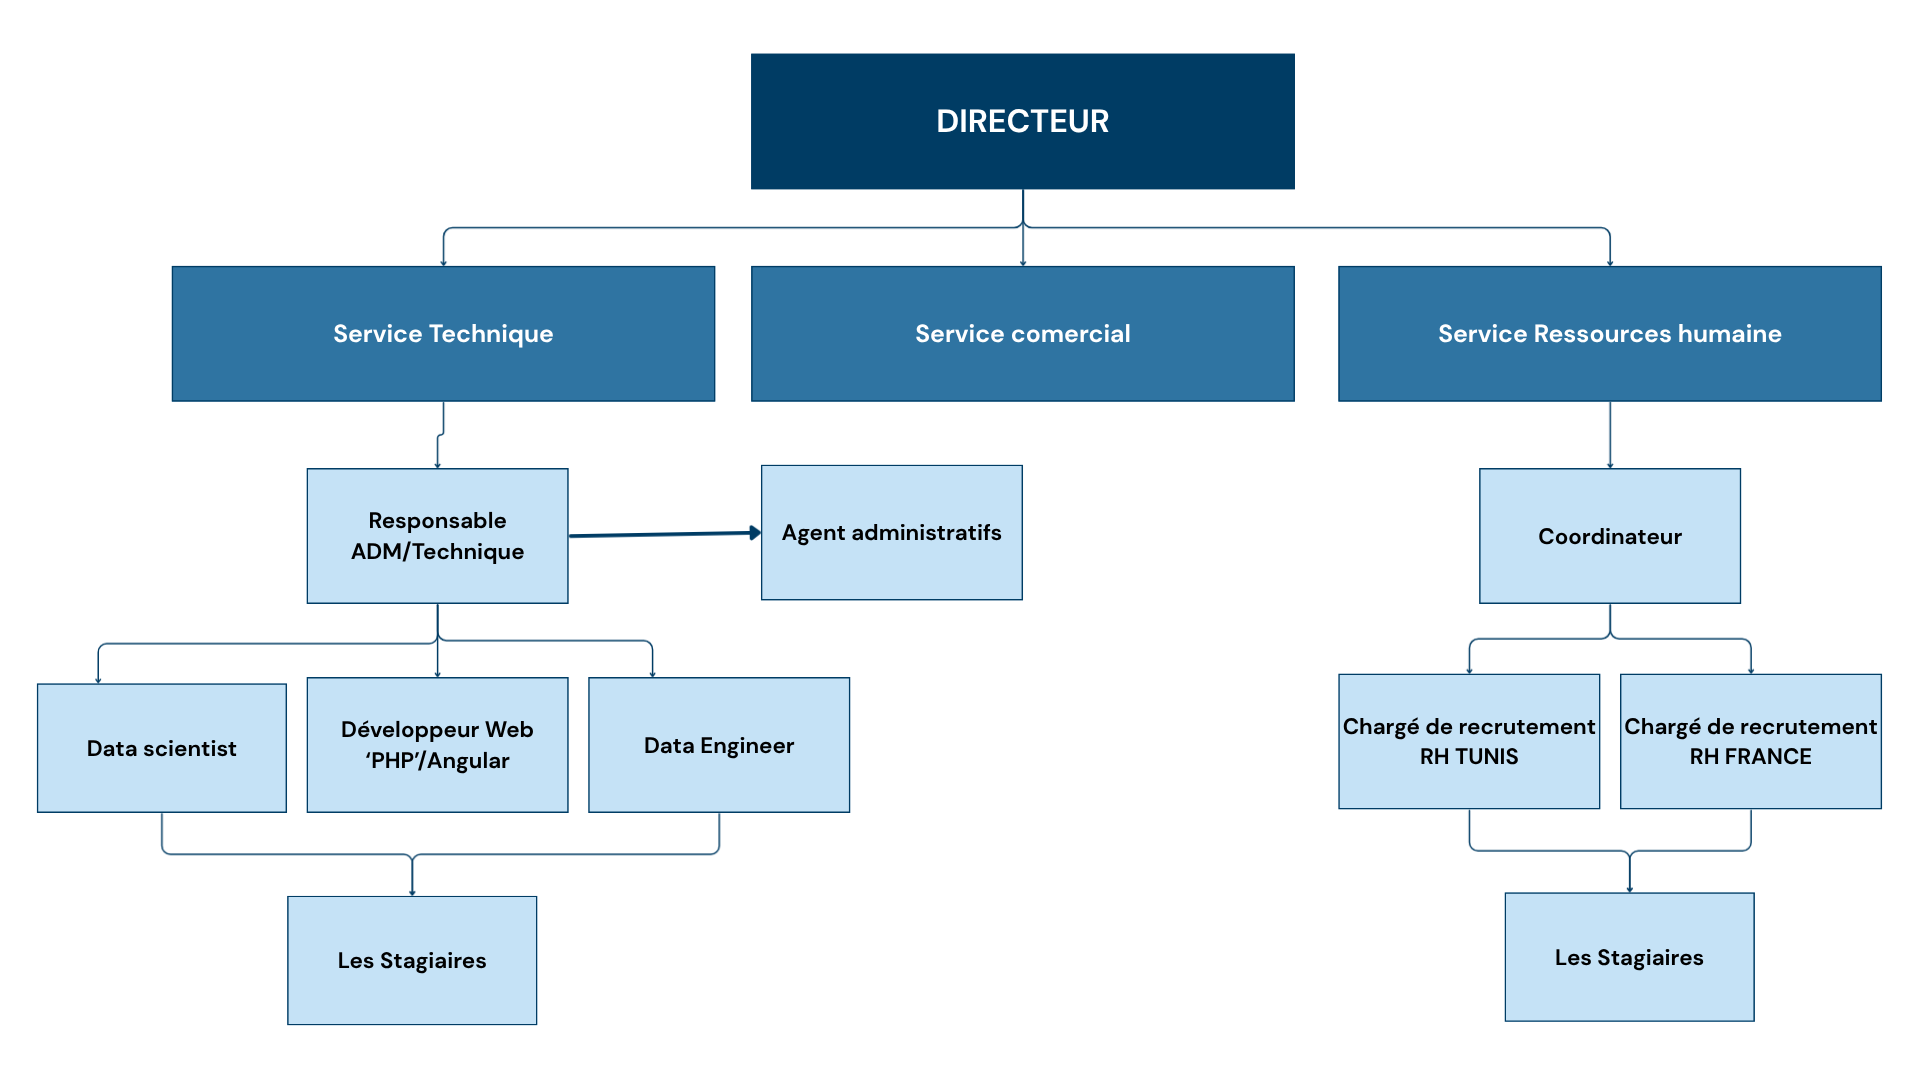
\includegraphics[width=\textwidth]{organigramme.png}
\caption{Organigramme de l'entreprise Smart-Conseil}
\label{fig:organigramme}
\end{figure}

\section{Étude de l'existant}

Le harcèlement scolaire est un phénomène grave et répandu.
Selon la DGESCO (Direction Générale de l'Enseignement Scolaire, service du Ministère de l'Éducation nationale français), environ 800~000 élèves sont victimes de harcèlement scolaire chaque année en France \cite{dgesco2023}.
Avec la généralisation d'Internet, ce phénomène prend désormais une dimension numérique : le cyberharcèlement.
Selon une étude publiée en 2024, 84,7\% des jeunes âgés de 15 à 24 ans passent en moyenne 3h50 par jour en ligne, et 58\% d'entre eux utilisent quotidiennement les réseaux sociaux \cite{digital2024}.

Face à ce problème, plusieurs solutions ont été développées :

\begin{itemize}
    \item Des lignes téléphoniques d'écoute et des questionnaires remplis manuellement par les élèves.
    \item Des outils de signalement intégrés aux plateformes de réseaux sociaux.
    \item \textbf{SafeBar} \cite{safebar} : un outil numérique développé par l'association e-Enfance qui permet de détecter des situations de cyberharcèlement à partir de signalements.
          Il est destiné aux établissements scolaires et aux parents souhaitant surveiller les activités en ligne.
          Il intervient après l'identification d'une victime et ne propose pas de mécanisme de détection préventive.
    \item \textbf{Stop Bashing!} \cite{stopbashing} : une application mobile permettant à un enfant de prendre une capture d'écran d'un message harcelant et de l'envoyer immédiatement à ses parents ou à un adulte référent.
          Le processus de signalement reste entièrement manuel.
    \item \textbf{Netethic} \cite{netethic} : une plateforme numérique développée par Smart-Conseil, dédiée à la détection et à la gestion du harcèlement en milieu scolaire.
          Elle offre un tableau de bord interactif pour visualiser les cas qui demandent l'attention des responsables, un système de gestion et de suivi des signalements, des outils d'analyse et une interface d'administration dédiée aux équipes pédagogiques.
\end{itemize}

\section{Critique de l'existant}

Ces solutions présentent des limites qui laissent plusieurs besoins sans réponse :

\begin{itemize}
    \item \textbf{Disponibilité limitée :} les services d'écoute et de signalement ne sont pas automatisés.
          Les utilisateurs ne peuvent obtenir de l'aide qu'aux heures ouvrées.
    \item \textbf{Barrière psychologique :} une victime peut hésiter à s'adresser directement à un adulte, par crainte des représailles ou de la stigmatisation.
    \item \textbf{Réactivité insuffisante :} un délai important s'écoule entre le signalement et la prise en charge effective de la victime.
    \item \textbf{Absence de support automatisé sur Netethic :} la plateforme ne dispose pas d'un assistant virtuel pour informer les visiteurs extérieurs, ni d'un outil de support automatisé pour le personnel, ni d'un mécanisme de soutien pour les élèves en difficulté, ni d'une analyse automatique des textes soumis.
\end{itemize}

\section{Solution envisagée}

Notre projet s'inscrit dans la plateforme \textbf{Netethic} et a pour objectif d'enrichir cette dernière par quatre modules intelligents et complémentaires basés sur l'intelligence artificielle.
Ces modules répondent directement aux besoins identifiés :

\begin{enumerate}
    \item \textbf{Assistant virtuel public (Noa) :} un assistant conversationnel disponible sur le site de Netethic en français et en anglais, accessible à toute heure, sans intervention humaine.
          Il répond aux questions des visiteurs sur la plateforme, ses fonctionnalités et ses tarifs.
          Il accompagne également les prospects qui souhaitent planifier une démonstration en collectant leurs coordonnées.
          Sa disponibilité continue élimine la dépendance aux horaires du personnel et garantit un accueil permanent des visiteurs.
    \item \textbf{Assistant de support interne :} un assistant destiné au personnel des établissements utilisant Netethic.
          Il répond aux questions sur les fonctionnalités de la plateforme, gère les demandes de rendez-vous et recueille les signalements de dysfonctionnements techniques.
    \item \textbf{Module de soutien émotionnel :} un système qui détecte les signaux de détresse dans les messages des utilisateurs et génère des réponses empathiques adaptées, en orientant l'utilisateur vers les ressources disponibles sur la plateforme.
    \item \textbf{Classificateur de harcèlement :} un système d'analyse automatique des textes qui identifie les types de comportements nécessitant une attention particulière, en s'appuyant sur les références juridiques françaises en vigueur.
\end{enumerate}

\section{Pipeline du projet}

Le projet suit un processus de développement structuré en plusieurs phases :

\begin{enumerate}
    \item \textbf{Phase préalable — Recherche et étude :} recherche bibliographique, analyse des solutions existantes et recueil des besoins auprès des parties prenantes.
    \item \textbf{Collecte et préparation :} recueil des documents de référence (contenu du site Netethic, documentation interne, textes de loi français).
    \item \textbf{Conception :} modélisation de l'architecture générale et des flux de traitement de chaque module.
    \item \textbf{Développement :} implémentation des modules à l'aide de cadres de développement spécialisés en intelligence artificielle.
    \item \textbf{Validation :} tests de performance, évaluation de la qualité des réponses et retours utilisateurs.
\end{enumerate}

\section{Méthodologie}

Pour gérer ce projet, nous avons adopté le cadre Scrum \cite{scrumguide}.
Scrum est une méthode agile de gestion de projet particulièrement adaptée au travail en équipe à distance.
Elle divise le travail en périodes courtes appelées sprints ; chaque sprint dure une semaine et se termine par une révision des résultats obtenus.

\begin{itemize}
    \item \textbf{Daily stand-ups (réunions quotidiennes) :}
          chaque jour, une courte réunion sur Microsoft Teams permet de discuter des objectifs, de l'avancement et des difficultés rencontrées.
    \item \textbf{Sprint Reviews (révisions de sprint) :}
          chaque semaine, une réunion d'équipe permet d'évaluer les tâches réalisées et de planifier le sprint suivant.
\end{itemize}

La modélisation du système a été réalisée avec le langage UML (Unified Modeling Language — langage de modélisation unifié), en utilisant l'outil Power AMC pour la création des diagrammes.

\section*{Conclusion}

Ce chapitre a présenté le cadre général du projet.
Nous avons décrit l'entreprise Smart-Conseil et son domaine d'activité.
Nous avons analysé les solutions existantes face au harcèlement scolaire et mis en évidence leurs limites.
Nous avons ensuite décrit les quatre modules que notre projet apporte à la plateforme Netethic, ainsi que le pipeline de développement et la méthode de gestion adoptés.

Dans le chapitre suivant, nous détaillons la spécification des besoins du système.
